% IE 643 course project report -- Team Binary_Brains
% Built on the official IE643_Project_Report.tex template (header, margins, section order unchanged).

\documentclass[twoside,english]{article}
\setlength{\oddsidemargin}{0.25 in}
\setlength{\evensidemargin}{-0.25 in}
\setlength{\topmargin}{-0.6 in}
\setlength{\textwidth}{6.5 in}
\setlength{\textheight}{8.5 in}
\setlength{\headsep}{0.75 in}
\setlength{\parindent}{0 in}
\setlength{\parskip}{0.1 in}

%
% ADD PACKAGES here:
%

\usepackage{amsmath,amsfonts,graphicx,algorithm,caption}
\usepackage[noend]{algpseudocode}
\usepackage{hyperref}
\usepackage{natbib}
\usepackage[document]{ragged2e}
\usepackage{graphicx} %package to manage images
\usepackage{amsmath}
\usepackage{mathtools}
\usepackage{xcolor}
\usepackage{booktabs}
\usepackage{float}
\usepackage{url}
\usepackage{tikz}
\usetikzlibrary{arrows.meta,positioning}

\newcounter{lecnum}
\renewcommand{\thepage}{\arabic{page}}
\renewcommand{\thesection}{\arabic{section}}
\renewcommand{\theequation}{\arabic{equation}}
\renewcommand{\thefigure}{\arabic{figure}}
\renewcommand{\thetable}{\arabic{table}}
\makeatletter
\def\BState{\State\hskip-\ALG@thistlm}
\makeatother

\newcommand{\lecture}[4]{
   \pagestyle{myheadings}
   \thispagestyle{plain}
   \newpage
   \setcounter{page}{1}
   \noindent
   \begin{center}
   \framebox{
      \vbox{\vspace{2mm}
    \hbox to 6.28in { {\bf IE 643: Deep Learning - Theory and Practice
		\hfill July-Dec 2026} }
       \vspace{4mm}
       \hbox to 6.28in { {\Large \hfill Project Report: #1  \hfill} }
       \vspace{2mm}
       \vspace{2mm}
       \hbox to 6.28in { {\it Team Name: #2 \hfill Team Members: #3} }
      \vspace{2mm}}
   }
   \end{center}
   \vspace*{4mm}
}
\renewcommand{\cite}[1]{[#1]}
\def\beginrefs{\begin{list}%
        {[\arabic{equation}]}{\usecounter{equation}
         \setlength{\leftmargin}{2.0truecm}\setlength{\labelsep}{0.4truecm}%
         \setlength{\labelwidth}{1.6truecm}}}
\def\endrefs{\end{list}}
\def\bibentry#1{\item[\hbox{[#1]}]}
\newcommand{\fig}[3]{
			\vspace{#2}
			\begin{center}
			Figure #1:~#3
			\end{center}
	}
\newtheorem{theorem}{Theorem}[lecnum]
\newtheorem{lemma}[theorem]{Lemma}
\newtheorem{proposition}[theorem]{Proposition}
\newtheorem{claim}[theorem]{Claim}
\newtheorem{corollary}[theorem]{Corollary}
\newtheorem{definition}[theorem]{Definition}
\newenvironment{proof}{{\bf Proof:}}{\hfill\rule{2mm}{2mm}}
\newcommand{\R}{\mathbb{R}}
\newcommand{\relL}{\mathrm{relL2}(D)}

\begin{document}
\lecture{PINN-based Inversion of Spatially-Varying Diffusivity}{Binary\_Brains}{24b2451, 24b2443}

\begin{center}
Jash Taparia (24b2451) \quad $\cdot$ \quad Mihir Gune (24b2443)\\[1mm]
Code repository: \url{https://github.com/bloodrepaer/IE643-Binary-Brains-PINN-Inversion} \citep{teamrepo}
\end{center}

\begin{abstract}
We recover an unknown, spatially varying diffusivity $D(x,y)$ in the two-dimensional heat equation $u_t=\nabla\cdot(D\nabla u)$ from sparse, noisy temperature sensors, and compare a physics-informed neural network (PINN) with classical PDE-constrained optimisation solved by the adjoint method. All data are synthetic. A hand-built finite-volume forward solver (5-point flux form, RK4, Crank--Nicolson and forward Euler, measured orders 4.03 / 2.01 / 1.00) generates 389 benchmark datasets from six families of ground-truth $D$, with controlled sensor count, layout, timing, horizon and noise. The classical baseline uses an exact discrete adjoint of Crank--Nicolson with L-BFGS-B and a discrepancy-principle regularisation weight, and was run on all 389 datasets. The PINN uses Fourier-feature networks for temperature and $\log D$ with a five-term physics-informed loss. When the initial and boundary conditions are known exactly and there are up to a few hundred sensors, the adjoint is more accurate: it wins 20/20 representative datasets (median $\relL$ 0.23 vs 0.47) and 41/44 datasets in a sensor $\times$ noise $\times$ layout sweep. The PINN wins in three regimes that we identified and tested with matched controls: (i) an unknown boundary condition or heat source, where the standard adjoint must assume one and fails (PINN better on 21 of 22 such datasets, median $\relL$ 0.38 vs 5.0); (ii) very dense sensor data, where a neural PINN reaches 8.6\% coefficient error at 7{,}500 sensors and 5\% noise against 25.1\% for a matched neural adjoint; (iii) too few sensors, where it degrades gracefully to the best constant instead of inventing structure. A Streamlit interface lets a user generate, select or upload sensor data, run both methods, and see the metrics and recovered maps.
\end{abstract}

\section{Introduction}

Many engineering and biomedical problems need a material property that cannot be measured directly: the thermal conductivity map of a composite plate with defects, the permeability of tissue, or the diffusivity of a drug through a hydrogel. What can be measured is the process that the property governs, here a temperature (or concentration) field $u(x,y,t)$, at a handful of sensor locations and times. Recovering the property from such data is an \emph{inverse problem}. Unlike the forward problem, it is ill-posed: many coefficient fields explain the same sparse readings, and small noise can produce large errors in the estimate.

Two families of methods address it. \emph{Classical PDE-constrained optimisation} represents the unknown with a finite set of parameters, solves the PDE exactly with a numerical solver at every iteration, and obtains the gradient of the data misfit from an adjoint solve \citep{vogel2002,plessix2006}. \emph{Physics-informed neural networks} \citep{raissi2019} represent the solution, and here also the coefficient, by neural networks, and encourage the PDE through a residual penalty computed by automatic differentiation. PINNs need no mesh, no adjoint derivation and no exact boundary data, which makes them attractive for messy real problems; whether they are also more accurate is an empirical question. The course project asks us to build both methods on the same synthetic data and to find where the PINN is better.

The rest of the report is organised as follows. Section~\ref{sec:workflow} gives the project workflow. We survey the literature in Section~\ref{sec:litsurvey}. Our approaches, split into work before and after the prep-presentation review, are in Section~\ref{sec:our_proj}, and the datasets in Section~\ref{sec:data}. Experiments and results are in Sections~\ref{sec:exp} and~\ref{sec:results}. The plan for novelty assessment is in Section~\ref{sec:Plan for Novelty Assessment}, and Section~\ref{sec:conclusion} concludes.

\section{Project Workflow} \label{sec:workflow}

\begin{itemize}
\item \textbf{Problem definition.} Fixed the PDE (divergence form), domain, initial and boundary conditions, unknown ($\log D$), metrics and the six ground-truth families.
\item \textbf{Literature review.} PINNs for inverse problems \citep{raissi2019}, PINNs for spatially varying diffusivity \citep{thakur2024}, adjoint vs PINN comparisons \citep{zhang2026}, spectral bias and Fourier features \citep{rahaman2019,tancik2020}.
\item \textbf{Forward solver and dataset (Deliverable 1).} Finite-volume solver with three time integrators, verified for order of accuracy; 389-dataset benchmark with nested sensors and controlled noise.
\item \textbf{Classical baseline (Deliverable 3).} Discrete adjoint of Crank--Nicolson, gradient verified by Taylor tests; run on all 389 datasets.
\item \textbf{PINN (Deliverable 2).} Two-network PINN, loss-weight sweep, 10-case benchmark.
\item \textbf{Head-to-head experiments (Deliverables 5, 6).} 20-dataset study and a 44-dataset sensor/noise/layout sweep, both methods on identical data.
\item \textbf{Where should a PINN win? (Deliverable 4).} Hypothesis suites H1--H9 with matched controls (sparse sensors, unknown BC, unknown source, heavy noise, long horizons, dense data, fine features); neural-coefficient campaign where both methods share the same $D$ network; dense-sensor sweep up to 10{,}000 sensors.
\item \textbf{Interface and packaging.} Streamlit app with upload, generation, both solvers, metrics and model reload; documented code and trained models.
\end{itemize}

\begin{figure}[H]
\centering
\begin{tikzpicture}[node distance=7mm and 6mm, box/.style={draw, rounded corners, align=center, font=\footnotesize, minimum height=13mm, text width=25mm, fill=blue!4}]
\node[box] (p) {Problem \&\\literature};
\node[box, right=of p] (f) {Forward solver\\(FV; RK4, CN, FE)};
\node[box, right=of f] (d) {389 synthetic\\datasets};
\node[box, right=of d] (c) {Classical adjoint\\inversion};
\node[box, below=of c] (n) {PINN\\inversion};
\node[box, left=of n] (e) {Head-to-head\\experiments};
\node[box, left=of e] (h) {Where a PINN\\wins (H1--H9,\\dense sensors)};
\node[box, left=of h] (i) {Interface,\\report,\\packaging};
\draw[-{Latex}] (p)--(f); \draw[-{Latex}] (f)--(d); \draw[-{Latex}] (d)--(c);
\draw[-{Latex}] (c)--(n); \draw[-{Latex}] (n)--(e); \draw[-{Latex}] (e)--(h); \draw[-{Latex}] (h)--(i);
\end{tikzpicture}
\caption{Project workflow from problem statement to deliverables.}\label{fig:workflow}
\end{figure}

\section{Literature Survey} \label{sec:litsurvey}

\textbf{Physics-informed neural networks.} Raissi, Perdikaris and Karniadakis \citep{raissi2019} train a network $u_\theta(x,t)$ on a loss that adds the data misfit to the mean squared PDE residual at collocation points, computed by automatic differentiation. Unknown PDE parameters are trained jointly with $\theta$, so the same framework solves forward and inverse problems. Two known difficulties shaped our design: networks learn low frequencies first (spectral bias, \citep{rahaman2019}), which random Fourier feature embeddings mitigate \citep{tancik2020}; and the gradients of the different loss terms can be badly unbalanced, so loss weights matter a great deal \citep{wang2021}.

\textbf{PINNs for spatially varying diffusivity.} Thakur et al. \citep{thakur2024} is the closest published work. They use two networks, one for concentration and one for $D(x,y)$, train on concentration fields of four test cases, use the divergence form $\nabla\cdot(D\nabla c)$, and also propose a backward-Euler consistency loss between consecutive snapshots. They report 4.6--6.3\% coefficient error on dense data and 6.45\% with 250 points. This motivated our two-network PINN design.

\textbf{Adjoint versus PINN.} Zhang, Alla and Karniadakis \citep{zhang2026} compare the two paradigms on Burgers, Darcy and Allen--Cahn problems while holding physics and data fixed. Their conclusion is that the adjoint is preferable when a reliable discrete solver exists and the unknown is low-dimensional, while PINNs become competitive when the unknown is itself a neural field, when the problem is high-dimensional (adjoint storage and solve costs grow quickly), or when the data are very noisy. They also recommend a PINN warm start for the adjoint.

\textbf{Classical inverse problems.} Our baseline follows standard reduced-space optimisation \citep{vogel2002}: Tikhonov or total-variation \citep{rudin1992} regularisation, gradients from the adjoint-state method \citep{plessix2006}, bound-constrained L-BFGS-B \citep{byrd1995}, and the regularisation weight chosen by Morozov's discrepancy principle \citep{morozov1966}. The Crank--Nicolson time stepping uses a Rannacher start \citep{rannacher1984} to damp stiff modes from a non-smooth initial state.

\section{Proposed Approach or Approaches} \label{sec:our_proj}

\textbf{Problem.} On $\Omega=[0,1]^2$ and $t\in[0,T]$,
\begin{equation}
\frac{\partial u}{\partial t}=\nabla\cdot\big(D(x,y)\nabla u\big) = D\,\Delta u + \nabla D\cdot\nabla u, \qquad u(\cdot,0)=u_0,\quad u|_{\partial\Omega}=g(t). \label{eq:pde}
\end{equation}
Given noisy readings $d_i = u(x_i,y_i,t_i)+\varepsilon_i$, $\varepsilon_i\sim\mathcal N(0,\sigma^2)$, we estimate $D>0$. We always work with $m=\log D$, which keeps $D$ positive and treats relative errors symmetrically. We keep the divergence form: the $\nabla D\cdot\nabla u$ term carries the information about where $D$ changes.

\subsection{Work done before prep-presentation review}

\begin{itemize}
\item Problem formulation, literature review and the plan: forward solver, synthetic dataset, classical adjoint baseline, PINN, and a hybrid PINN$\rightarrow$adjoint method.
\item First forward solver: Crank--Nicolson with a 9-point stencil, data simulated on the same grid used for inversion.
\item First dataset version: absolute noise $\sigma\in\{0.01, 0.05\}$, eight random observation times per file, seeds from Python's \texttt{hash()}.
\end{itemize}

The review exposed weaknesses that we fixed afterwards (Table~\ref{tab:changes}).

\begin{table}[H]
\centering\footnotesize
\begin{tabular}{p{4.3cm}p{4.3cm}p{6.5cm}}
\toprule
Prep presentation & Final & Reason \\
\midrule
9-point stencil & 5-point flux form, harmonic-mean links & 1.3--1.8$\times$ more accurate on every family; simpler exact adjoint \\
Crank--Nicolson only & RK4, Crank--Nicolson, forward Euler behind one interface & RK4 generates data, CN is the inversion solver, FE is a benchmark \\
Data on the inversion grid & Data on $129^2$, inversion on $65^2$ & Avoids the ``inverse crime'' \\
Absolute noise 0.01 / 0.05 & Relative noise $\eta\in\{0,1,5,10\%\}$ & Absolute $\sigma$ was 30--280\% of the signal \\
8 random times per file & Fixed time protocols + temporal-density sweep & Reproducible; time becomes a controlled axis \\
\texttt{hash()} seeds & \texttt{zlib.crc32} seeds + manifest & \texttt{hash()} changes every Python run \\
Hybrid PINN$\rightarrow$adjoint planned & Dropped & Scope; compute spent on more experiments \\
\bottomrule
\end{tabular}
\caption{Changes made after the prep-presentation review.}\label{tab:changes}
\end{table}

\subsection{Work done after prep-presentation review}

\subsubsection{Forward solver}
Space is discretised with node-centred finite volumes on an $N\times N$ grid. Each link between neighbouring nodes $p,q$ carries the harmonic mean $2D_pD_q/(D_p+D_q)$, because the two half-cells act as thermal resistances in series. Eliminating the Dirichlet boundary nodes gives the semi-discrete system $\dot{\mathbf u}=L(D)\mathbf u+\mathbf b(t)$ with $L$ sparse, symmetric and negative definite. Three integrators share this operator: RK4 (data generation), Crank--Nicolson with two backward-Euler half-steps at the start (Rannacher start; used for inversion and replay; unconditionally stable) and forward Euler (benchmark only). The Crank--Nicolson matrix is factorised once per $D$ and reused for every forward and adjoint step.

\subsubsection{Classical inversion: discrete adjoint}
The unknown is $m=P\theta$, where $\theta$ lives on a $16\times16$ control grid and $P$ is bilinear interpolation to the $65\times65$ inversion grid; $D=e^m$ with bounds $10^{-3}\le D\le 10$. We minimise
\begin{equation}
J(\theta)=\frac{1}{2\sigma^2}\big\|Q\,\mathbf u(m)-\mathbf d\big\|^2+\alpha R(m),\qquad R_{\rm Tik}=\tfrac12\!\int|\nabla m|^2,\quad R_{\rm TV}=\int\!\sqrt{|\nabla m|^2+\epsilon},
\end{equation}
where $\mathbf u(m)$ is the Crank--Nicolson solution (a hard constraint) and $Q$ interpolates bilinearly in space and linearly in time, so sensors and times may be off-grid. The gradient with respect to all 256 parameters comes from one forward and one backward (adjoint) sweep that mirrors the time stepping exactly, including the Rannacher steps. We optimise with L-BFGS-B ($\le150$ iterations per $\alpha$), starting from the best constant $D$, over a decreasing continuation $\alpha_k=N_d\,10^{-k/2}$ with warm starts. $\alpha$ is chosen by the discrepancy principle: the first $\alpha$ whose RMS misfit is at most $\sigma$.

\subsubsection{PINN}
\textbf{Architecture.} The temperature network maps $(x,y,t)$ through random Fourier features (scale 0.35) to three hidden \texttt{tanh} layers of 80 units (19{,}521 parameters). Its output is an analytic heat-kernel approximation of the initial bumps plus a learned correction multiplied by $16x(1-x)y(1-y)$ and $\tanh(8t/T)$, so the zero boundary and the initial condition hold by construction. The coefficient network maps $(x,y)$ through Fourier features to three \texttt{tanh} layers of 64 units (12{,}545 parameters) and outputs a correction to a trainable background $\log D$, tapered to the background near the walls, with $D=\exp(\mathrm{clamp}(m,-5,2))$. We use \texttt{tanh} because the loss needs second derivatives, and ReLU networks have zero curvature almost everywhere.

\textbf{Loss.}
\begin{equation}
\mathcal L = 40\,\mathcal L_{\rm data}+20\,\mathcal L_{\rm PDE}+10\,\mathcal L_{\rm BC}+20\,\mathcal L_{\rm IC}+\lambda\,R(\log D).
\end{equation}
$\mathcal L_{\rm data}$ is the mean squared misfit normalised by the mean squared reading, damped once it falls within $0.95\sigma^2$ so the network does not chase the noise. $\mathcal L_{\rm PDE}$ is the mean squared residual of $u_t-(D_xu_x+D_yu_y+D\Delta u)$ at 768 collocation points per step. 90\% of its gradient is routed to the $D$ network and 10\% to the $u$ network, so the PDE mostly shapes $D$ rather than distorting $u$. $R$ is Tikhonov ($\lambda=2\times10^{-4}$, smooth families) or TV ($3\times10^{-4}$, sharp families).

\textbf{Training.} AdamW \citep{kingma2015,loshchilov2019} (weight decay $10^{-5}$), learning rates $1.5\times10^{-3}$ ($u$) and $3.5\times10^{-3}$ ($D$) with cosine annealing to $10^{-5}$, gradient clipping at 1.0, 1{,}500 epochs. The $D$ network's rate is held near zero for about 50 epochs and ramped over 15\% of training, so $u$ fits the data first. We keep the best checkpoint from the last 35\% of training. Implemented in PyTorch \citep{paszke2019}.

\textbf{Boundary-aware variant.} To test unknown boundary conditions, \texttt{pinn\_inversion\_bc.py} reads the boundary mode from the problem file. With a known non-zero boundary it replaces the hard zero window by a soft boundary loss. With an unknown boundary (\texttt{free}) it has no window and no boundary loss, so wall values are determined only by the data and the PDE.

\subsubsection{Neural-coefficient extension}
The grid adjoint and the PINN differ in two ways at once: how $D$ is represented (16$\times$16 grid vs network) and how the physics is enforced (exact solver vs penalty). To separate them, we built a shared coefficient network (\texttt{NeuralDiffusivity}), a float64 \texttt{tanh} MLP with 3 layers of 32 units whose output $z_\phi(x,y)$ is mapped to a bounded coefficient,
\begin{equation}
\log D=\log D_{\min}+\log(D_{\max}/D_{\min})\,\mathrm{sigmoid}(z_\phi),\qquad D\in[10^{-3},10].
\end{equation} Its last layer is initialised to reproduce the best constant fitted to the data. Both methods use it with the same seed:
\begin{itemize}
\item \textbf{Neural adjoint}: the same Crank--Nicolson solver and discrete adjoint give $\partial J/\partial m$ on the grid, which is back-propagated through the network (a vector--Jacobian product); optimised with L-BFGS-B.
\item \textbf{Neural PINN}: a temperature MLP trained jointly with the same $D$ network on data and PDE residual (Adam followed by L-BFGS).
\end{itemize}
For the dense-sensor study we used matched temporal variants. The PINN's state network has hard initial and boundary conditions and a backward-Euler consistency defect on 4{,}096 random time pairs ($\Delta t/T=0.01$). The adjoint uses backward Euler with 100 full steps. Both use $\alpha=1$ and seed 42, and run 1{,}000 Adam steps followed by $10\times400$ self-scaled Broyden (SSBroyden) quasi-Newton iterations, as in \citep{zhang2026}.

\subsubsection{Interface}
The interface is a Streamlit \citep{streamlit} web app (\texttt{app/streamlit\_app.py}) over a thin backend (\texttt{app/core.py}) that calls the project's solvers unchanged. It has four tabs.
\begin{enumerate}
\item \textbf{Data.} Three ways to get sensor data: generate a synthetic dataset (any of 17 $D$ fields or an uploaded $D$ map; horizon; 5--100 sensors or the full field; layout; time protocol; noise; boundary condition; seed); pick one of the 389 benchmark datasets; or upload a CSV of readings \texttt{x,y,t,u[,sigma]}, optionally with an initial condition and a true $D$ for scoring.
\item \textbf{Run.} Classical settings (control grid 8--32, Tikhonov/TV, iterations) and PINN settings (100--6{,}000 epochs, regulariser, weight, seed).
\item \textbf{Results.} The displayed metrics: replay RMS$/\sigma$ for both methods, plus $\relL$ and the best-constant baseline when the truth is known. Also maps on a shared colour scale, $\log(\hat D/D)$ error maps, profiles, the $\alpha$-selection curve, a sensitivity map, PINN loss curves, and downloads (trained models, $\hat D$ as CSV/NPZ, metrics, figures).
\item \textbf{Load model.} Reload a saved \texttt{classical\_model.npz} or \texttt{pinn\_best.pt}, or one of 40 bundled trained models. The app rebuilds $D$ from the model file and scores it.
\end{enumerate}
Design choices: every data source is written to the project's own dataset format, so both solvers read user data exactly as they read the benchmark. Generation reuses the benchmark generator, so interface data are statistically identical to the benchmark. Uploads are validated (columns; $x,y\in[0,1]$; $t>0$). Both estimates are scored by replaying $\hat D$ through the same Crank--Nicolson solver. Results stay in session state, so switching tabs never retrains. Every path was tested headlessly with \texttt{streamlit.testing} and in a browser (Figure~\ref{fig:interface}).

\section{Data set Details} \label{sec:data}

All data are synthetic and generated by our own code, so no data were downloaded from external websites. One command, \texttt{python generate\_dataset\_v2.py} (about 4 minutes on a laptop CPU), writes the benchmark \texttt{datasets\_v2\_rk4\_zero/}: 389 datasets and 35 ground-truth simulations, 175\,MB.

\textbf{Ground-truth fields.} Six families plus 11 variants: A smooth sinusoid; B Gaussian bump; C circular inclusion (sharp edge; high/low-contrast variants); D layered (and coarse/fine checkerboards); E Gaussian random field (short/long correlation variants); F plate with defects (single, many, small, voids, low contrast).

\textbf{Generation steps.}
\begin{enumerate}
\item Build the true $D$ on the $129^2$ data grid; the inversion-grid truth is every second node.
\item For each horizon (Fourier number) $\mathrm{Fo}\in\{0.02,0.05,0.1,0.2\}$ set $T=\mathrm{Fo}/\bar D$. The initial condition is two Gaussian bumps; the boundary is held at zero (other scenarios: heated, ramped or pulsed edge).
\item Simulate $u$ with RK4 on $129^2$ at its largest stable step; store 401 output times and 41 snapshots.
\item Fix one noise level per (family, Fo, $\eta$): $\sigma=\eta\times$ RMS of a reference signal.
\item Choose sensors from a fixed pool of 100 per (family, layout), so sets are nested ($5\subset20\subset50\subset100$). Layouts are random, grid, clustered and boundary-only.
\item Choose observation times from a protocol: \texttt{uniform4}$\ldots$\texttt{uniform200}, \texttt{log8}, \texttt{early8}, \texttt{late8}, \texttt{final1}.
\item Interpolate the clean field at each (sensor, time) and add Gaussian noise with seed \texttt{crc32(name)}.
\end{enumerate}

\textbf{Sweeps.} S1 sensors $\{5,20,50,100,\text{full}\}\times$ noise $\{0,1,5,10\%\}$; S2 horizon $\times$ time protocol; S3 time density $\times$ noise; S4 layout $\times\{20,50\}$ sensors. That is 63 datasets per main family $\times$ 6, plus 11 variant baselines, for 389 in total. Dataset keys read \texttt{<family>\_\_Fo<Fo>\_\_<protocol>\_\_n<count>\_\_<layout>\_\_eta<$\eta$>}.

\textbf{Format.} \texttt{problem/} holds the PDE, $T$, the initial condition and the boundary values. \texttt{sensors/<key>.csv} has columns \texttt{x,y,t,u,sigma}, one row per reading (also the interface upload format). \texttt{ground\_truth/} holds the true $D$ and snapshots, used only for scoring. A manifest records every configuration and seed. No further pre-processing is applied. The methods read the readings directly, and the PINN normalises time by $T$.

\textbf{Additional collections} (same format, generated by scripts in the package): the hypothesis suites H1--H5 (57 datasets) and H6/H7/H9 (24), each with matched controls; a nested density extension (180 configurations, 5--3{,}969 sensors on the inversion grid, 1/5/10\% noise); and dense sets of 1{,}000--10{,}000 sensors sampled from the $129^2$ simulation.

\begin{figure}[H]
\centering
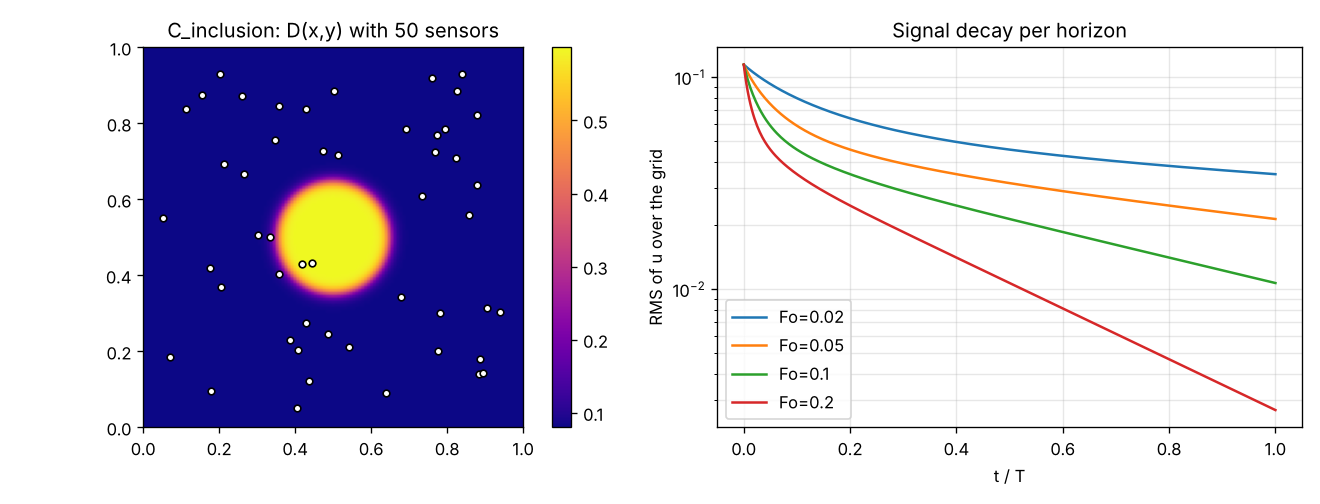
\includegraphics[width=0.78\textwidth]{figs/C_inclusion_overview.png}\\
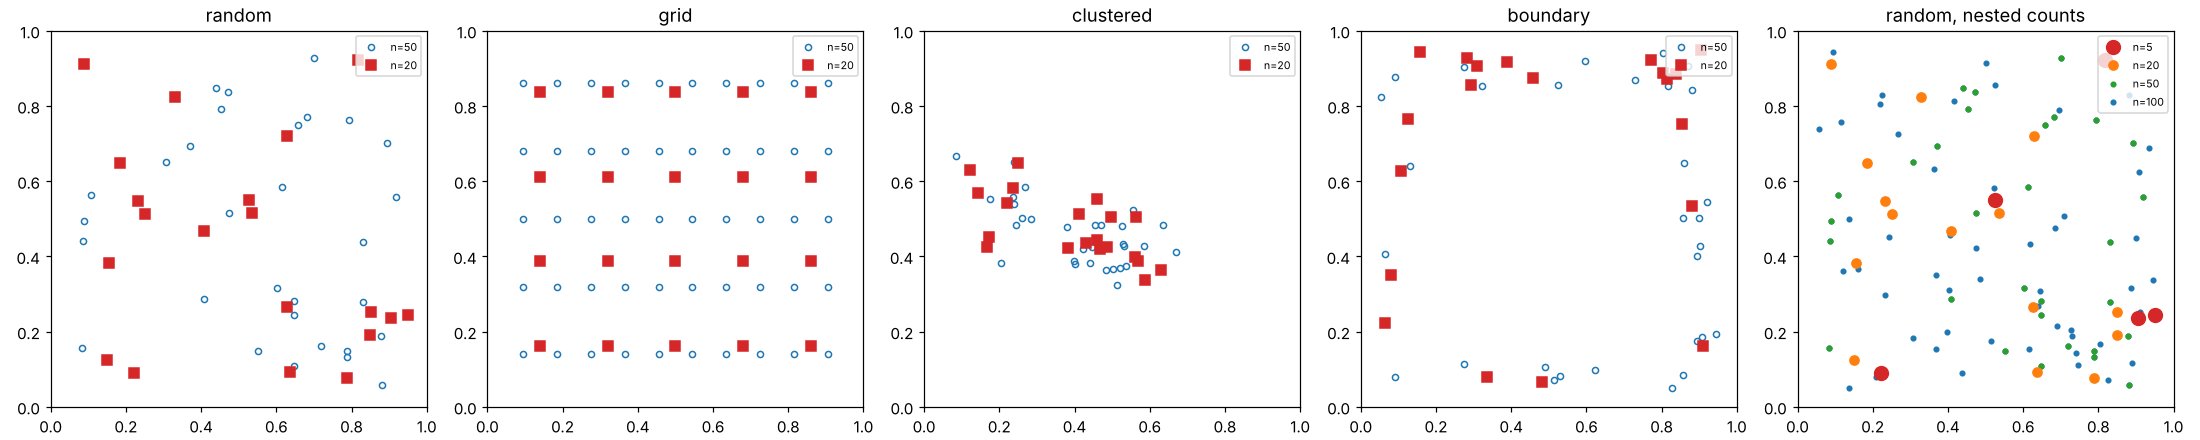
\includegraphics[width=0.9\textwidth]{figs/sensor_layouts.png}
\caption{Top: inclusion family with 50 random sensors, and how fast the signal decays for each horizon. Bottom: the four sensor layouts.}\label{fig:data}
\end{figure}

\section{Experiments} \label{sec:exp}

\textbf{Metrics.} (1) $\relL=\|\hat D-D\|_2/\|D\|_2$ on the $65^2$ grid, the main ranking metric (lower is better). (2) Replay RMS$/\sigma$: $\hat D$ is run through the Crank--Nicolson solver and compared with the readings. About 1 means the data are explained to the noise level; much more than 1 means under-fitting, much less means over-fitting. This metric needs no ground truth, so it is the one shown to a user. (3) The best-constant baseline: the $\relL$ of the best single constant $D$. A method is useful only if it beats it.

\textbf{Code.} All code, trained models and results are in our GitHub repository \citep{teamrepo}, whose README maps every deliverable to its files:\\ \url{https://github.com/bloodrepaer/IE643-Binary-Brains-PINN-Inversion}

\textbf{Hardware.} The classical runs, the PINN benchmark and the 20/44-dataset studies ran on CPUs: a laptop, and 2-core cloud Linux containers with one thread per run. The neural campaign ran on a Windows laptop CPU, Kaggle notebooks (CPU, and GPU for some pilots) and Google Colab (T4 GPU). Wall times are therefore descriptive.

We list every experiment, including those with negative results.
\begin{enumerate}
\item \textbf{Verification.} Integrator order of accuracy against an exact-in-time matrix-exponential solution. Adjoint transpose identity, Taylor tests and finite-difference gradient checks (\texttt{test\_adjoint.py}). Problem-file sufficiency: replaying the true $D$ from the problem files alone.
\item \textbf{Classical inversion on all 389 datasets} (Tikhonov; TV also run on the inclusion and defect families).
\item \textbf{PINN loss-weight sweep}: 10 settings on the Gaussian bump (50 sensors, 5\% noise).
\item \textbf{20-dataset head-to-head study}: representative datasets across all families; identical data and identical scoring.
\item \textbf{Sensor $\times$ noise $\times$ layout sweep, both methods}: 44 datasets on the inclusion (C) and bump (B); 5/20/50/100 random sensors $\times$ 0/1/5/10\% noise, plus grid/clustered/boundary layouts at 20 and 50 sensors.
\item \textbf{Hypothesis suites ``where should a PINN win?''} (81 paired datasets): H1 very sparse sensors (3/5/8); H2 unknown boundary condition (heated, ramped or pulsed edge, not given to either method); H3 unknown internal heat source; H4 heavy noise (10--50\%); H5 long horizons; H6 more readings (100/400 sensors $\times$ 40 times); H7 unknown boundary with more readings; H9 features finer than the $16\times16$ control grid. Each test dataset has a control that differs only in the tested factor. For unknown physics both methods are told the same assumed model (zero boundary, no source).
\item \textbf{Neural-coefficient campaign}: neural adjoint on all 389 benchmark datasets plus the density and hypothesis collections; neural PINN on a canonical subset.
\item \textbf{Dense-sensor sweep}: 1{,}000/3{,}000/5{,}000/7{,}500 sensors $\times$ 1/5/10\% noise on the smooth field (12 paired cells, 24 fits), plus a 10{,}000-sensor reference pair. An advantage counts only if the fit completed, has lower $\relL$, and passes a pre-declared replay screen ($\le1.1\sigma$ under both Crank--Nicolson and backward Euler) checked before the truth was opened.
\end{enumerate}

\section{Results}\label{sec:results}

\subsection{Solver and adjoint verification}
Measured orders are 4.03 (RK4), 2.01 (Crank--Nicolson) and 1.00 (forward Euler) (Figure~\ref{fig:verif}). Just above their stability limits, RK4 and forward Euler blow up, which is why the inversion uses an implicit scheme. The adjoint passes all checks: transpose identity to $4\times10^{-16}$, Taylor slopes 1.996--2.000, and adjoint vs finite differences to $10^{-8}$. Replaying the true $D$ from the problem files alone gives median RMS$/\sigma=1.01$ over 296 noisy datasets, so the problem files are sufficient and the noise model is right.

\begin{figure}[H]
\centering
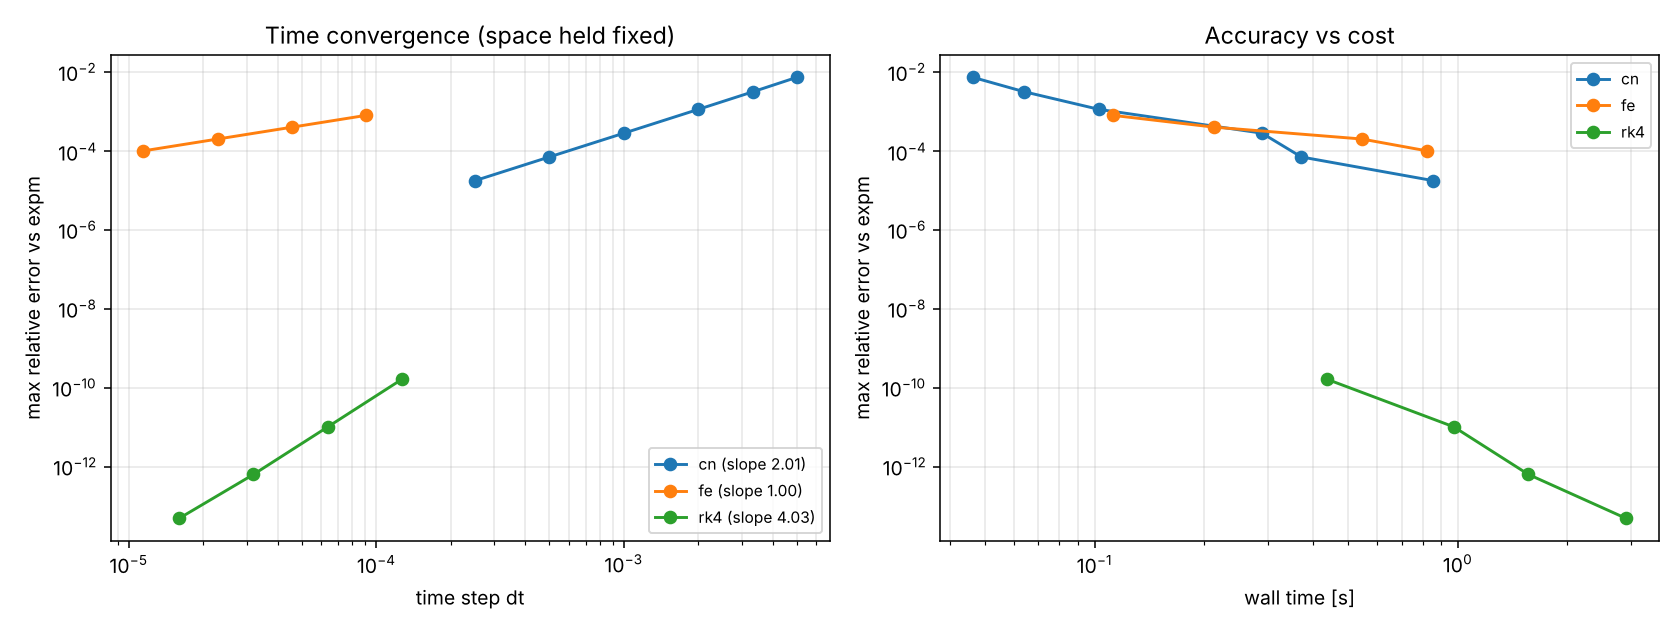
\includegraphics[width=0.62\textwidth]{figs/integrator_convergence.png}\hfill
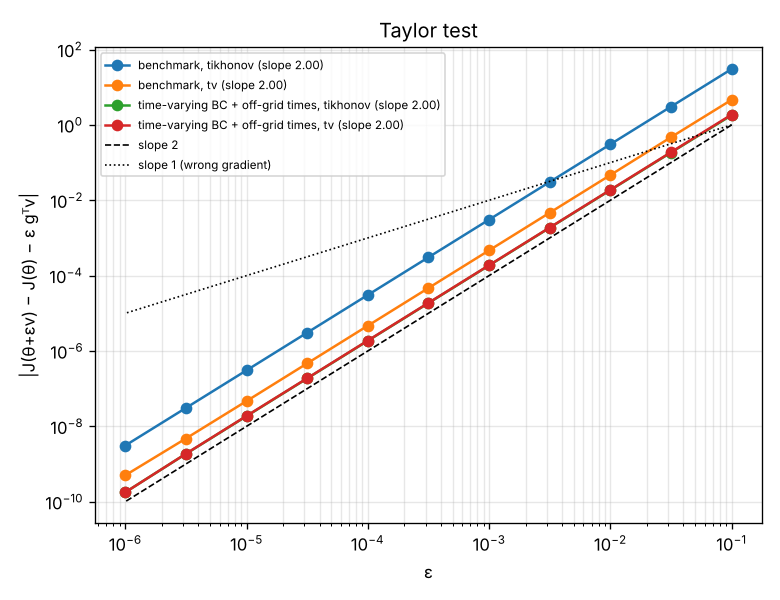
\includegraphics[width=0.33\textwidth]{figs/taylor_test.png}
\caption{Left: convergence of the three integrators. Right: Taylor test of the adjoint gradient; the remainder falls with slope 2.}\label{fig:verif}
\end{figure}

\subsection{Classical inversion on the benchmark}
The adjoint fits 324 of the 389 datasets to the noise level (median replay RMS$/\sigma=0.98$). Its error falls with more sensors, more snapshots and less noise (Table~\ref{tab:classical}). The inclusion is the hardest family: with 50 sensors it barely beats the best constant (0.66 vs 0.75), and full-field data bring it to 0.22. A negative result: on the layered field with $\le1\%$ noise, the discrepancy principle drives $\alpha$ very low, the method fits discretisation error at the sharp interfaces, and it overshoots (up to 1.40).

\begin{table}[H]
\centering\footnotesize
\begin{tabular}{lccccc|cccc}
\toprule
& \multicolumn{5}{c|}{Sensors (5\% noise)} & \multicolumn{4}{c}{Noise (50 sensors)}\\
Family & 5 & 20 & 50 & 100 & full & 0\% & 1\% & 5\% & 10\% \\
\midrule
A smooth & 0.319 & 0.128 & 0.103 & 0.110 & 0.077 & 0.060 & 0.075 & 0.103 & 0.135 \\
B bump & 0.394 & 0.289 & 0.229 & 0.189 & 0.075 & 0.014 & 0.119 & 0.229 & 0.317\\
C inclusion & 0.690 & 0.631 & 0.661 & 0.462 & 0.215 & 0.354 & 0.439 & 0.661 & 0.713\\
D layered & 0.211 & 0.319 & 0.216 & 0.240 & 0.149 & 1.404 & 0.975 & 0.216 & 0.300\\
E random field & 0.327 & 0.186 & 0.207 & 0.175 & 0.069 & 0.056 & 0.116 & 0.207 & 0.253\\
F defects & 0.236 & 0.193 & 0.182 & 0.160 & 0.112 & 0.113 & 0.118 & 0.182 & 0.201\\
\bottomrule
\end{tabular}
\caption{Classical adjoint, $\relL$ (Tikhonov, Fo 0.1, 8 uniform times, random sensors).}\label{tab:classical}
\end{table}

\subsection{PINN tuning}
Over 10 loss-weight settings on the bump, the best $\relL$ was 0.398 (equal weights, no regulariser) and an over-fitting setting (data weight 250, PDE weight 2) gave 0.873, against 0.229 for the adjoint. No setting came within 1.7$\times$ of the adjoint. More importantly, the network's own data fit was $\chi^2\approx0.95$ for nine very different $D$ estimates (0.40--0.65), while replaying those $D$ through the solver gave $\chi^2$ from 3 to 56. A PINN can fit the readings with the wrong coefficient. We therefore score every estimate by replaying it through the solver, never by the network's own fit.

\subsection{Head-to-head on representative datasets}
On 20 datasets the adjoint has the lower error on all 20, with a median ratio of 2.0$\times$ and median $\relL$ 0.23 vs 0.47 (Figure~\ref{fig:s20}). It beats the best constant on 20/20, the PINN on 8/20. Median replay RMS$/\sigma$ is 0.97 (adjoint) vs 3.7 (PINN), and median CPU time is 46\,s vs 125\,s. The gap is smallest where the problem is hardest for everyone (sharp inclusion, few sensors) and largest where data are rich (full field: 0.030 vs 0.405). The adjoint turns extra data into accuracy; the PINN does not, partly because its data term is a mean over readings.

\begin{figure}[H]
\centering
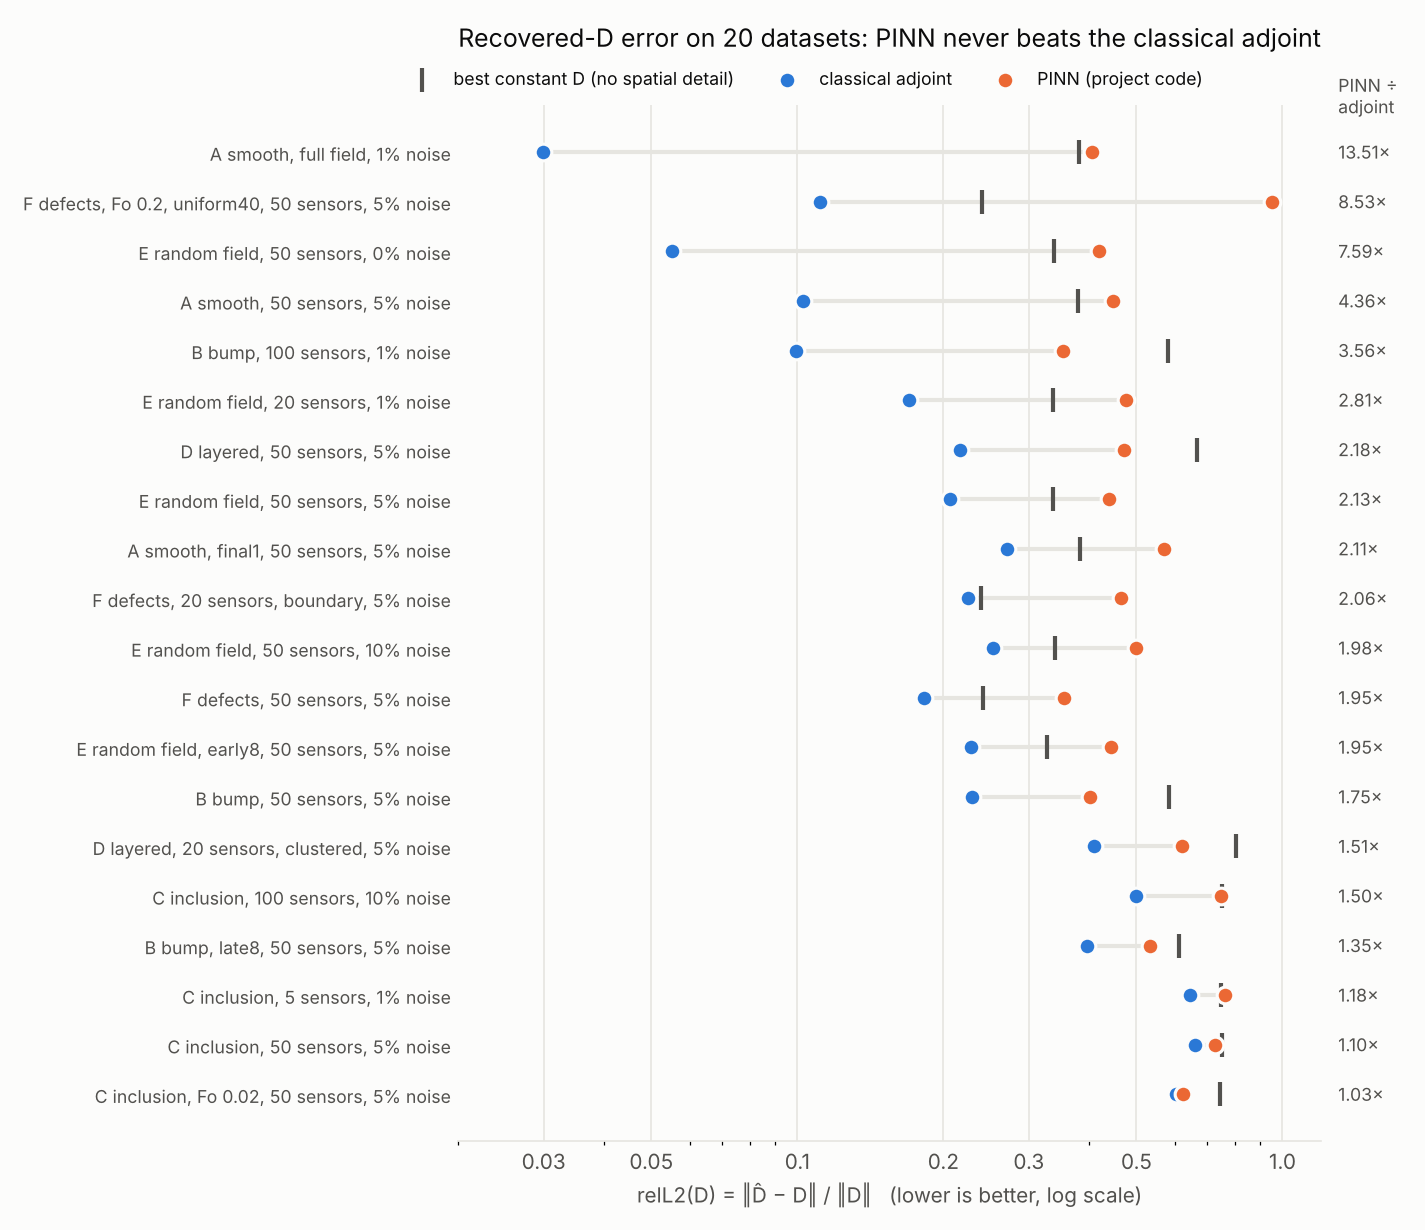
\includegraphics[width=0.49\textwidth]{figs/s20_relL2.png}\hfill
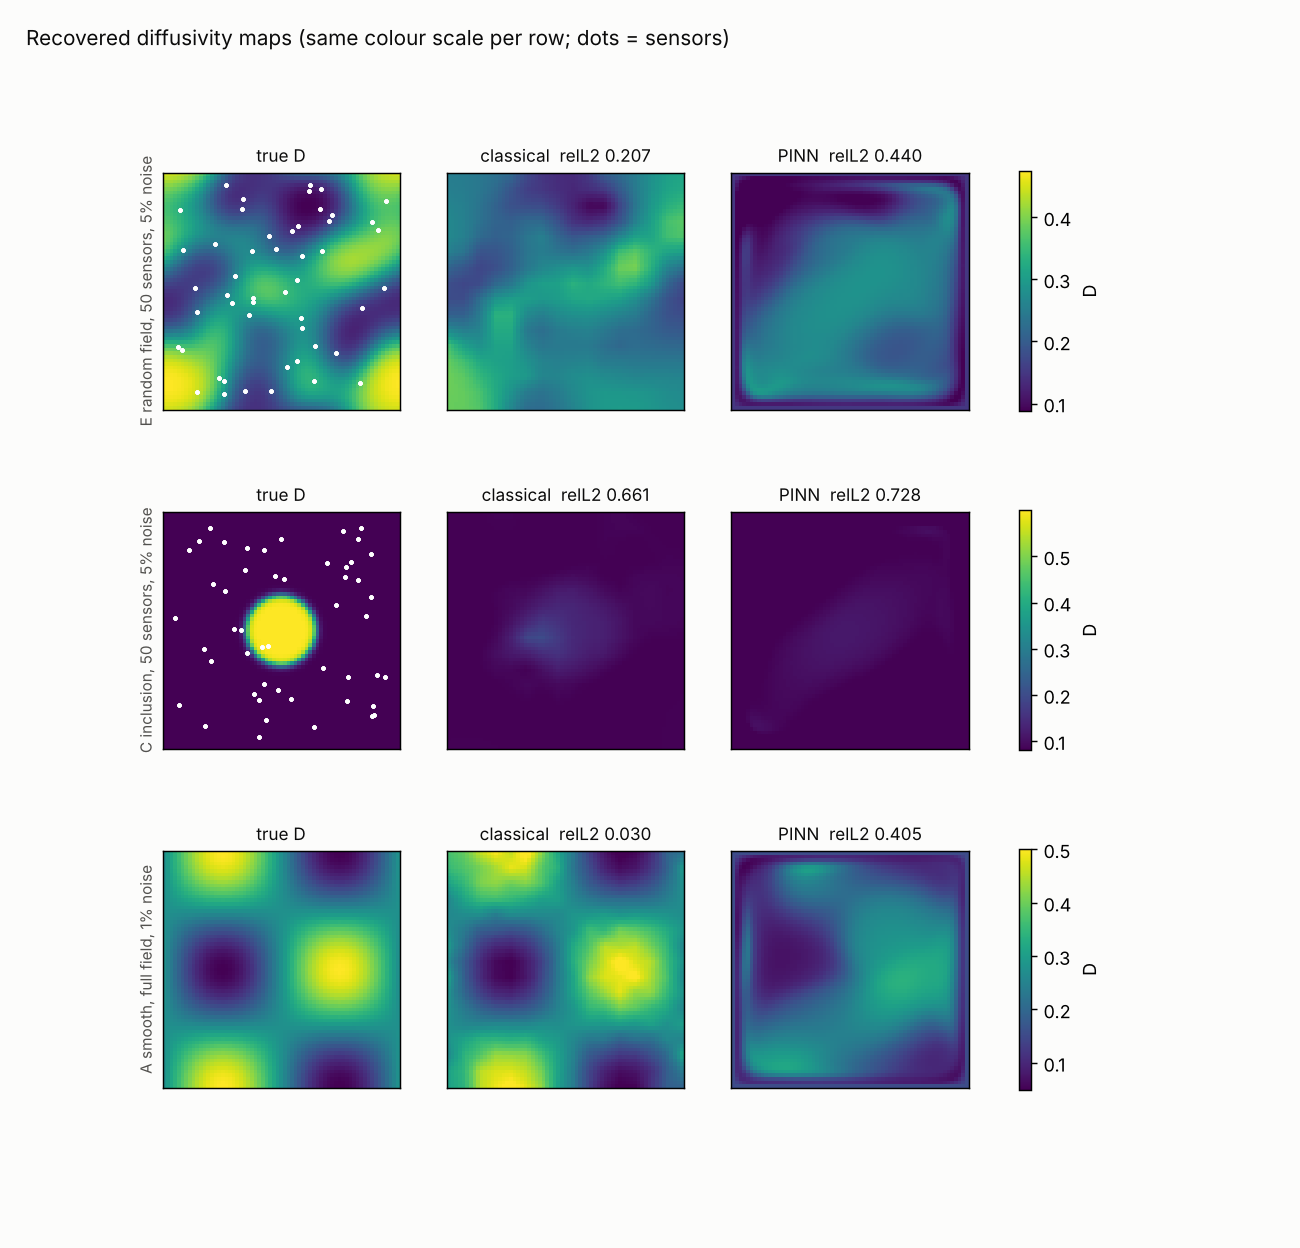
\includegraphics[width=0.49\textwidth]{figs/s20_fields.png}
\caption{Left: $\relL$ on 20 datasets (log scale; bars are the best constant). Right: recovered maps for three of them.}\label{fig:s20}
\end{figure}


\subsection{Sensor density, layout and noise (both methods)}
In the 44-dataset sweep the adjoint has the lower error on 41 (median $\relL$ 0.36 vs 0.61; best constant 0.68), see Figure~\ref{fig:sweep}. On the bump both methods improve with more sensors and less noise, and the adjoint is 1.2--24$\times$ better. On the inclusion the PINN stays at 0.68--0.76, within 10\% of the best constant, at every sensor count and noise level. The adjoint reaches 0.19--0.25 with 100 sensors at 1--5\% noise but is erratic below that. A grid layout beats random sensors on the bump for both methods (adjoint 0.116 vs 0.229 at 50 sensors), and boundary-only sensors are worst. The PINN's three wins are all on the inclusion with too little information: 5 random sensors at 5\% noise (0.746 vs 0.779), 20 boundary sensors (0.766 vs 1.529) and 50 boundary sensors (0.740 vs 0.747). There the PINN stays at the constant level while the adjoint fits noise and invents structure. This is graceful degradation, not a better reconstruction.

\begin{figure}[H]
\centering
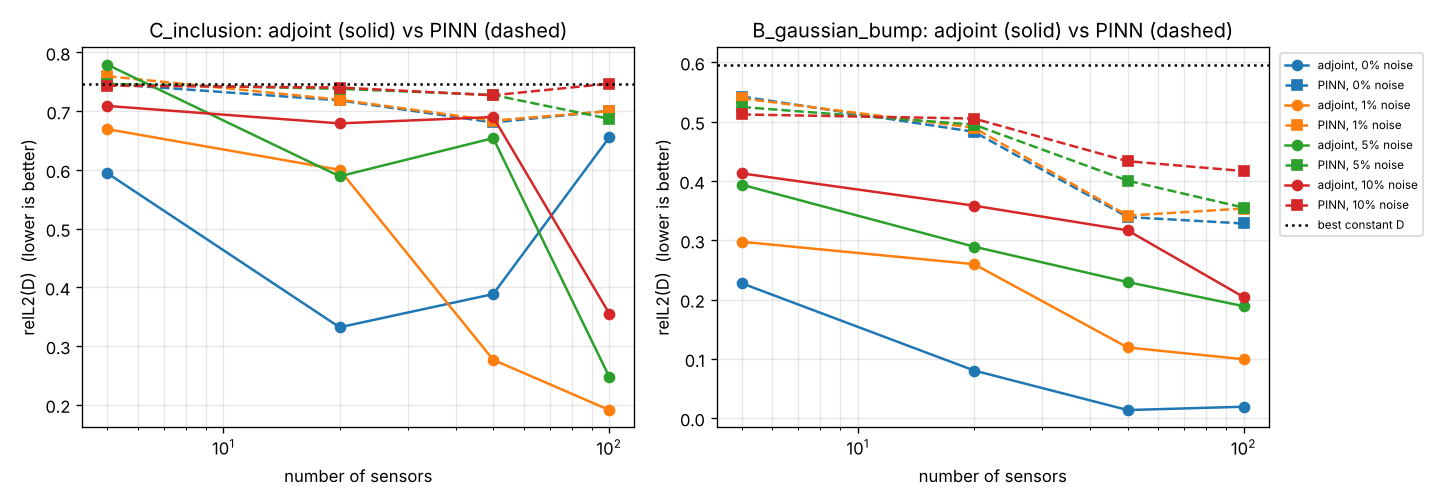
\includegraphics[width=0.95\textwidth]{figs/sweep_comparison.png}
\caption{$\relL$ against sensor count at four noise levels; adjoint solid, PINN dashed, best constant dotted.}\label{fig:sweep}
\end{figure}

\subsection{Where the PINN is better: hypothesis suites}
Table~\ref{tab:hyp} and Figure~\ref{fig:hyp} summarise the 81 paired hypothesis datasets. With the physics fully known (sparse sensors, heavy noise, long horizons, more data), the adjoint wins 58 of 59. With an \emph{unknown boundary condition or source}, the PINN wins 21 of 22. Figure~\ref{fig:misspec} shows why. Once the boundary is wrong, even the \emph{true} $D$ replays at about 9--21$\sigma$ under the assumed model, so an exact-constraint method must distort $D$ to explain the data (median $\relL$ 5.0). The PINN's soft PDE penalty, and in H2/H7 its free walls, absorb the mismatch, and it stays below the best constant (0.38 vs 0.58). This is a win over the standard adjoint formulation. A classical method that also inferred the boundary values or the source would be a stronger comparator, and we list it as future work.

\begin{table}[H]
\centering\footnotesize
\begin{tabular}{lccccc}
\toprule
Group & Datasets & PINN wins & Adjoint & PINN & Best const.\\
\midrule
Physics known (H1, H4--H6, H9, controls) & 59 & 1 & 0.123 & 0.412 & 0.344\\
BC or source unknown (H2u, H3u, H7u) & 22 & 21 & 5.011 & 0.379 & 0.580\\
\bottomrule
\end{tabular}
\caption{Hypothesis suites: number of PINN wins and median $\relL$. ``Unknown'' means withheld from both methods.}\label{tab:hyp}
\end{table}

\begin{figure}[H]
\centering
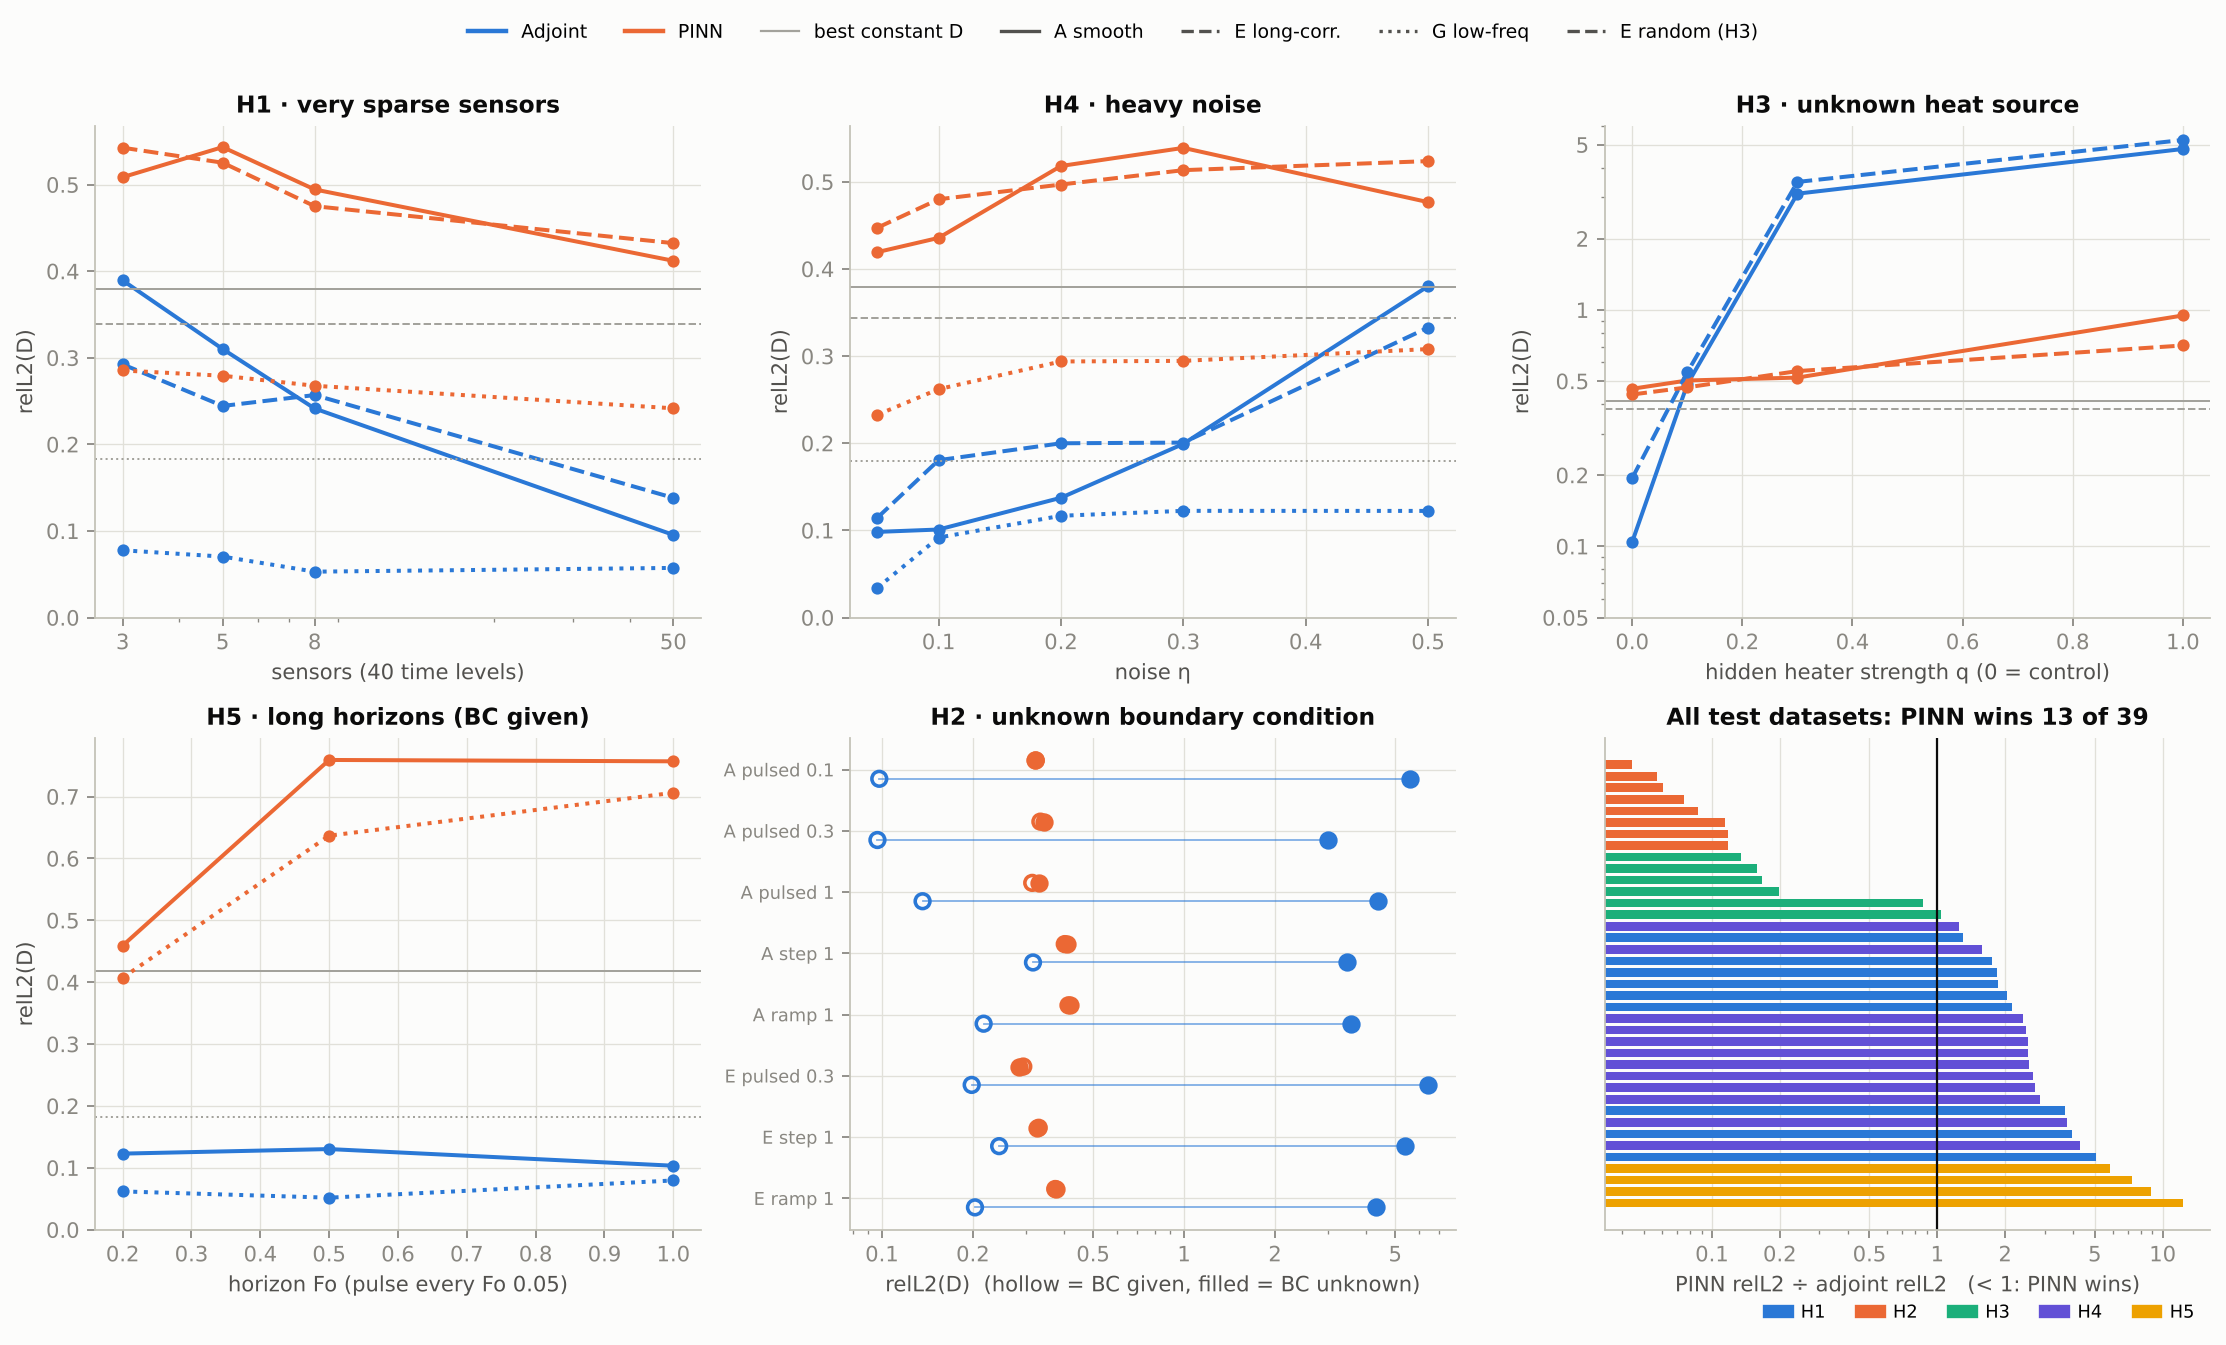
\includegraphics[width=0.95\textwidth]{figs/C1_pinnwin_comparison.png}
\caption{Hypothesis suites H1--H5. The PINN wins only where the boundary condition (H2) or heat source (H3) is unknown.}\label{fig:hyp}
\end{figure}

\begin{figure}[H]
\centering
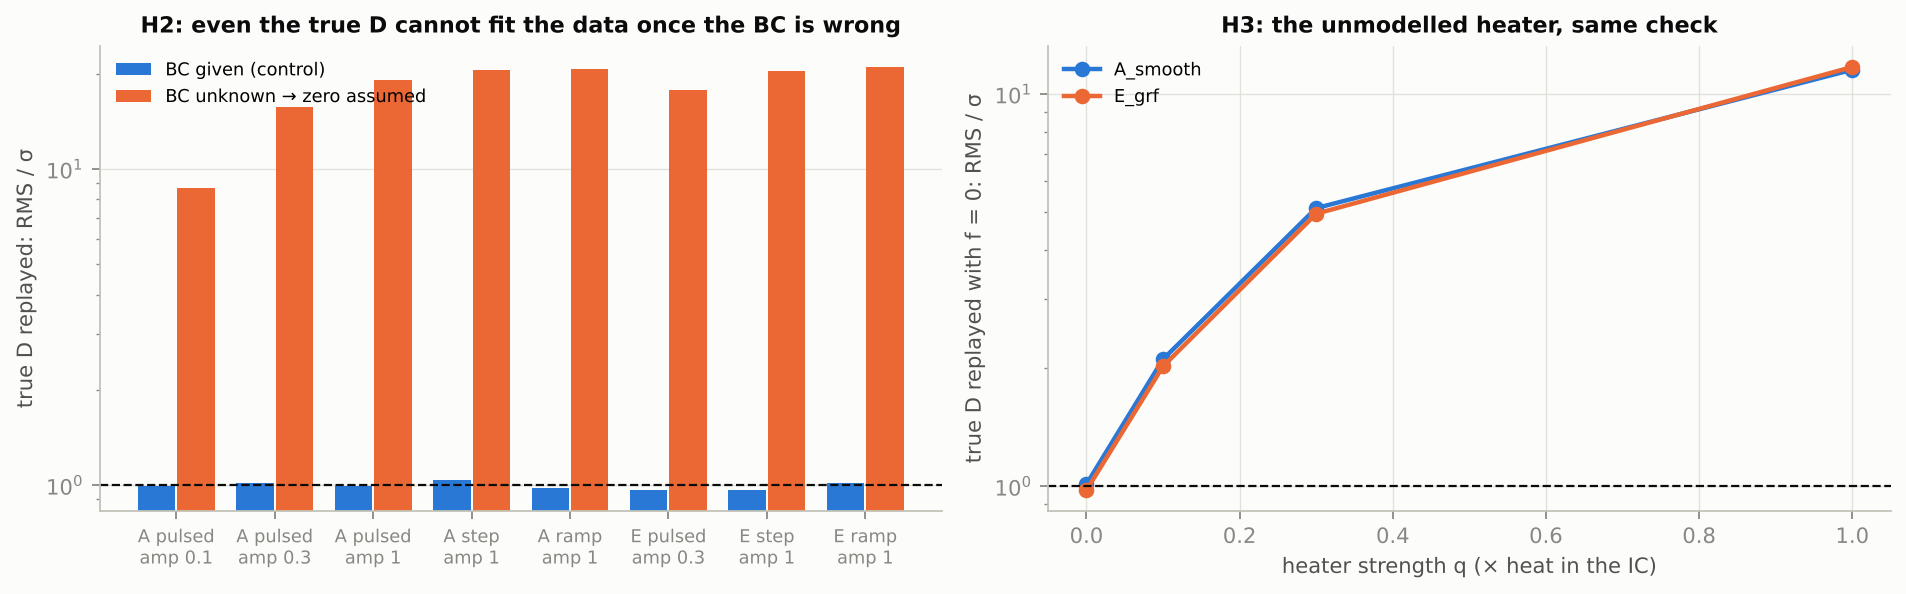
\includegraphics[width=0.85\textwidth]{figs/W2_misspecification_gap.png}
\caption{Why the adjoint fails under unknown physics: even the true $D$ cannot fit the data under the assumed boundary (left) or source (right).}\label{fig:misspec}
\end{figure}

\subsection{Neural coefficient and dense sensors}
Giving the adjoint the same neural representation of $D$ did not change its accuracy: the neural adjoint and the grid adjoint have median $\relL$ 0.226 vs 0.225 on the 389 benchmark datasets. With up to a few hundred sensors the neural PINN behaves like the original PINN. On canonical cases it fits the sensors but its $D$ replays at about 5.8$\sigma$ (median $\relL$ 0.61). The picture changes with very dense data (Table~\ref{tab:dense}, Figure~\ref{fig:dense}). At 5\% noise the PINN's error falls from 35.4\% (1{,}000 sensors) to 8.6\% (7{,}500), while the matched neural adjoint stays at 21--25\%. At 7{,}500 sensors both pass both replay screens, so this is a consistency-qualified PINN advantage. A 10{,}000-sensor reference pair gives 6.8\% vs 26.4\%. At 1\% noise the PINN has lower error at every density but fails the replay screens. At 10\% noise the adjoint is better up to 5{,}000 sensors; at 7{,}500 the PINN's error is slightly lower (22.6\% vs 23.3\%) but it fails the backward-Euler replay screen. These are single-field, single-seed results with capped optimisation, so they establish a regime worth studying, not a general rule.

\begin{table}[H]
\centering\footnotesize
\begin{tabular}{rr cc cc}
\toprule
Sensors & Noise & PINN $\relL$ & Adjoint $\relL$ & PINN replay CN / BE ($\sigma$) & Adjoint replay CN / BE ($\sigma$)\\
\midrule
1{,}000 & 5\% & 35.37\% & 21.45\% & 1.924 / 2.005 & 1.076 / 0.967\\
3{,}000 & 5\% & 16.48\% & 23.01\% & 1.136 / 1.150 & 1.095 / 0.992\\
5{,}000 & 5\% & 13.03\% & 23.79\% & 1.102 / 1.068 & 1.098 / 0.992\\
7{,}500 & 5\% & \textbf{8.62\%} & 25.09\% & 1.097 / 1.025 & 1.098 / 0.994\\
7{,}500 & 1\% & 5.61\% & 45.64\% & 2.969 / 1.873 & 2.595 / 1.068\\
7{,}500 & 10\% & 22.64\% & 23.26\% & 1.098 / 1.122 & 1.019 / 0.993\\
\bottomrule
\end{tabular}
\caption{Dense-sensor sweep (smooth field, temporal neural PINN vs backward-Euler neural adjoint). Replay is checked against $1.1\sigma$.}\label{tab:dense}
\end{table}

\begin{figure}[H]
\centering
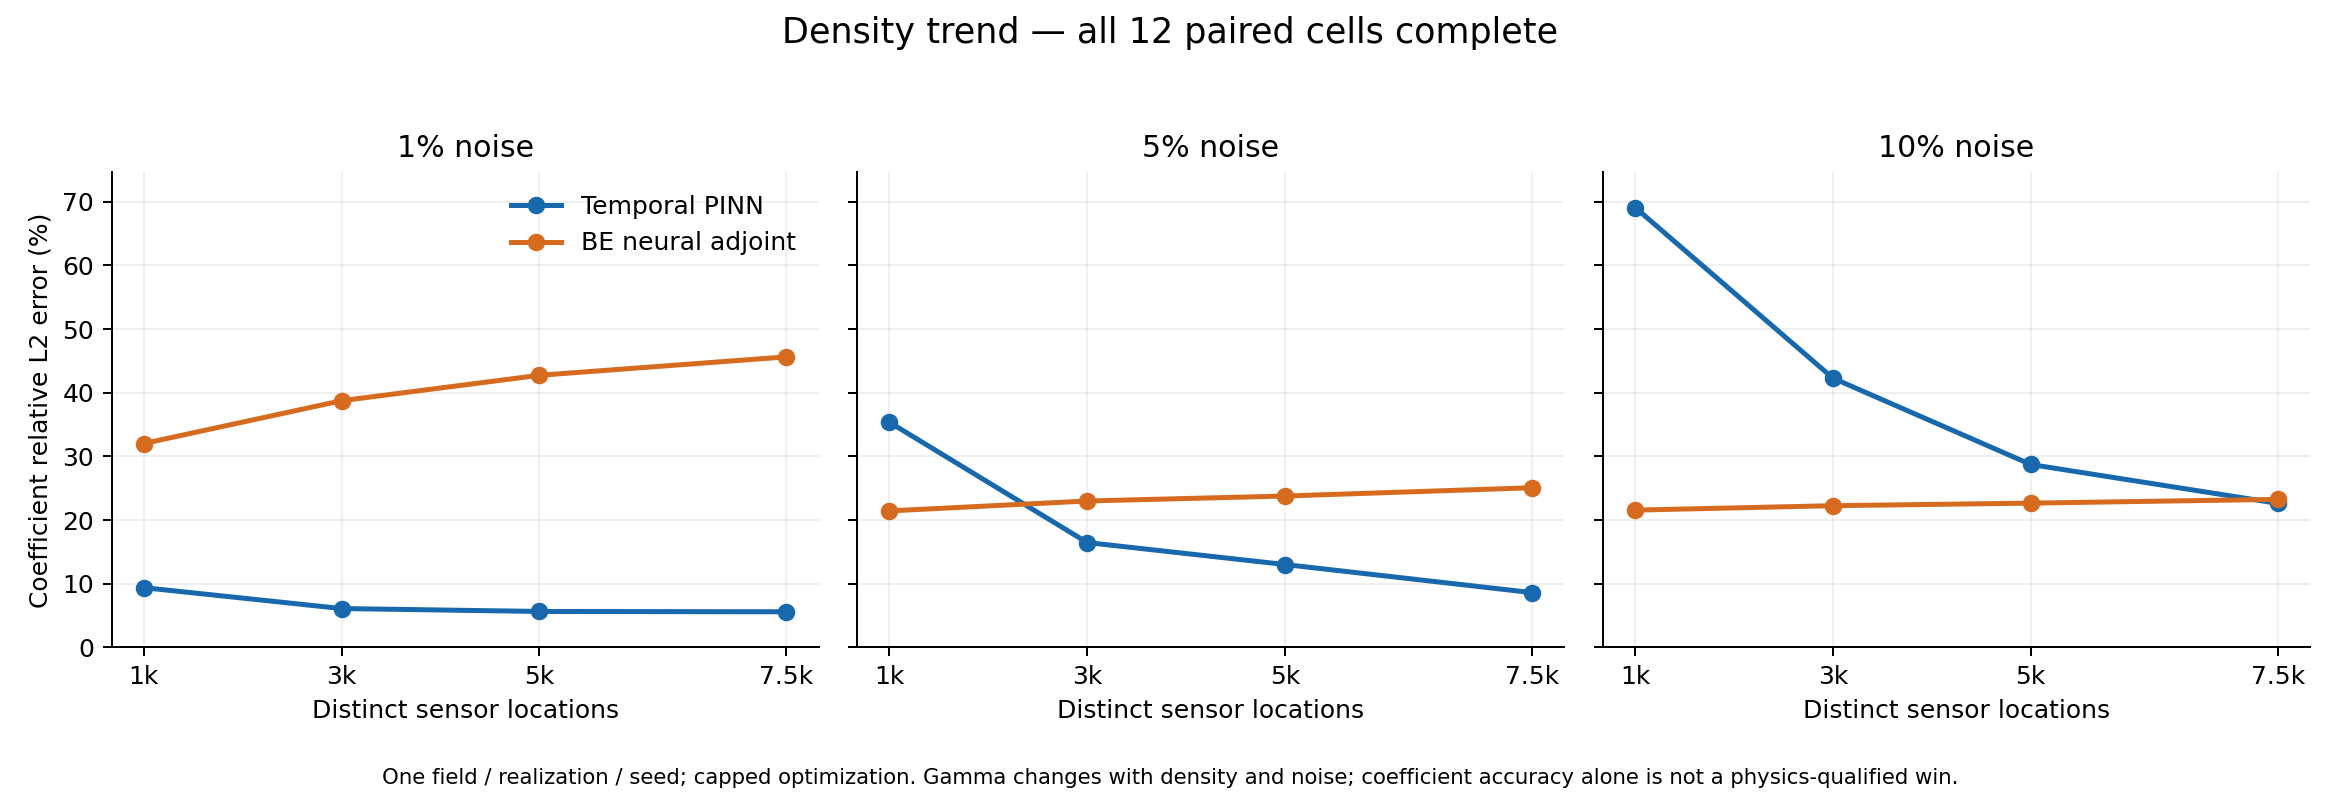
\includegraphics[width=0.95\textwidth]{figs/density_trend.png}
\caption{Coefficient error against sensor density at three noise levels (12 paired cells).}\label{fig:dense}
\end{figure}

\subsection{Interface}
Figure~\ref{fig:interface} shows the results tab for the inclusion dataset. Classical: $\relL$ 0.661, replay 0.98$\sigma$. PINN: 0.730, 2.38$\sigma$. Best constant: 0.751. The bundled models reproduce the stored comparison numbers when rescored in the app.

\begin{figure}[H]
\centering
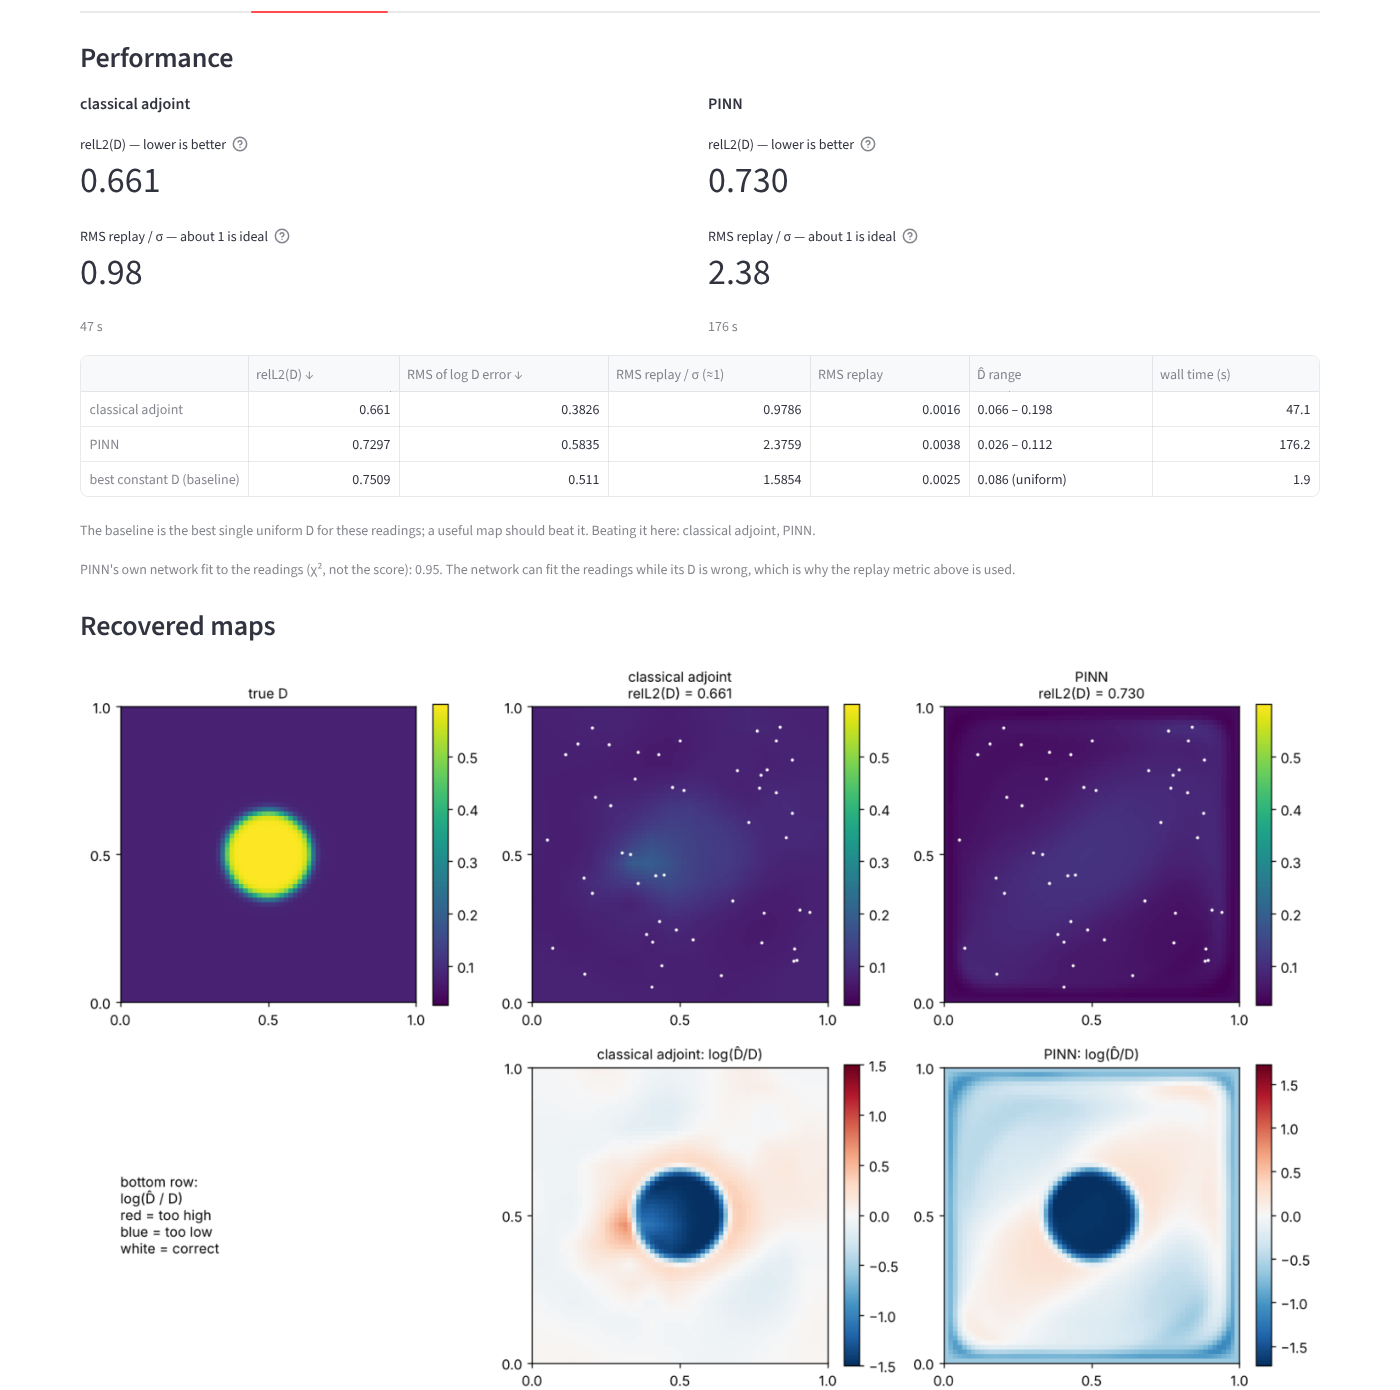
\includegraphics[width=0.72\textwidth]{figs/interface_results.png}
\caption{Interface results tab: displayed metrics, recovered maps and $\log(\hat D/D)$ error maps.}\label{fig:interface}
\end{figure}

\section{Plan for Novelty Assessment} \label{sec:Plan for Novelty Assessment}

\begin{enumerate}
\item \textbf{A fair classical comparator under unknown physics.} Add the boundary values (a few parameters per edge and time) and a low-dimensional source as extra unknowns in the adjoint, and re-run H2, H3 and H7. This tests whether the PINN's 21/22 advantage survives against a stronger baseline, or whether it is due to the standard formulation's rigidity.
\item \textbf{Hybrid PINN$\rightarrow$adjoint.} Use the PINN's $D$ (robust under unknown physics and dense data) to warm-start the adjoint, and measure total cost honestly, including the PINN's training time.
\item \textbf{Make the PINN use more data.} Replace the mean data loss by a $\sigma$-weighted sum, train in float64 with a quasi-Newton optimiser, and repeat the dense-sensor sweep over several fields and seeds to test whether the density advantage is general.
\item \textbf{Uncertain initial conditions}, known only at the sensors or with 5--10\% error. This is another regime where an exact-constraint method should suffer.
\item \textbf{Uncertainty quantification} for $\hat D$ from a Gauss--Newton Hessian (adjoint) or an ensemble of PINNs.
\end{enumerate}

\section{Conclusion} \label{sec:conclusion}

We built the full pipeline for recovering a spatially varying diffusivity from sparse, noisy heat data. It consists of a verified finite-volume forward solver and a 389-dataset benchmark, a classical adjoint inversion with exact gradients, a PINN, a neural-coefficient extension in which both methods share the same network for $D$, and an interface that runs both methods on generated, benchmark or uploaded data. In the standard setting (exact initial and boundary conditions, up to a few hundred sensors) the classical method is about twice as accurate, fits the data to the noise level, and is faster. Representing $D$ by a network does not change this. The PINN is the better choice in three regimes that we identified with matched controls: when the boundary condition or a heat source is unknown, when the data are very dense, and when the data are too sparse to identify $D$, where it degrades gracefully instead of overshooting. Its value is flexibility and robustness to imperfect physics rather than accuracy on a perfectly specified problem. Future work will test that advantage against a classical method that also infers the unknown physics, and combine the two methods.

\bibliographystyle{plain}
\bibliography{refs}

\end{document}
